% Source for docs/static/img/reinforce-baselines.svg. Rebuild from the repository root:
%   pdflatex -output-directory=/tmp docs/scripts/reinforce-baselines.tex
%   pdf2svg /tmp/reinforce-baselines.pdf docs/static/img/reinforce-baselines.svg
%   python3 docs/scripts/prepare_rollout_svgs.py
\documentclass[tikz,border=3pt]{standalone}
\usepackage{amsmath,amssymb}

% Sample colors match the joint-tree leaves; sign colors match the dark-theme map.
\definecolor{s1}{RGB}{255,140,0}
\definecolor{s2}{RGB}{255,180,200}
\definecolor{s3}{RGB}{0,180,100}
\definecolor{s4}{RGB}{0,180,220}
\colorlet{advpos}{blue!80!black}
\colorlet{advneg}{red!80!black}

% Return scale (pt per unit), column centers, and the shared returns R^k_t.
\def\s{32}
\def\returns{{0.1,0.4,0.7,0.4}}
\def\colx{{140,190,240,290}}

% \variantrow{axis y}{name}{mode}{baseline formula}{b1,b2,b3,b4}{spanning baseline or empty}
\newcommand{\variantrow}[6]{%
  \pgfmathsetmacro{\yo}{#1}
  \node[anchor=west] at (0,\yo+17) {\textbf{#2}\enspace{\scriptsize\texttt{#3}}};
  \node[anchor=west] at (0,\yo+3) {#4};
  \foreach \k [count=\i from 0] in {#5} {
    \pgfmathsetmacro{\x}{\colx[\i]}
    \pgfmathsetmacro{\r}{\returns[\i]}
    \pgfmathsetmacro{\a}{\r-\k}
    \pgfmathsetmacro{\yb}{\yo+\s*\k}
    \pgfmathsetmacro{\yr}{\yo+\s*\r}
    \fill[black, fill opacity=.07] (\x-8,\yo) rectangle (\x+8,\yr);
    \pgfmathtruncatemacro{\sgn}{\a>0.001 ? 1 : (\a<-0.001 ? -1 : 0)}
    \ifnum\sgn=1
      \fill[advpos, fill opacity=.4] (\x-8,\yb) rectangle (\x+8,\yr);
      \node[advpos] at (\x,\yo-8) {$+\pgfmathprintnumber[fixed,precision=1]{\a}$};
    \else\ifnum\sgn=-1
      \fill[advneg, fill opacity=.4] (\x-8,\yr) rectangle (\x+8,\yb);
      \node[advneg] at (\x,\yo-8) {$\pgfmathprintnumber[fixed,precision=1]{\a}$};
    \else
      \node at (\x,\yo-8) {$0$};
    \fi\fi
    \ifcase\i\def\c{s1}\or\def\c{s2}\or\def\c{s3}\or\def\c{s4}\fi
    \draw[\c, line width=.8pt] (\x-8,\yo) rectangle (\x+8,\yr);
    \ifx\relax#6\relax
      \ifdim\k pt>0pt
        \draw[black, line width=.6pt, dash pattern=on 2pt off 1.5pt] (\x-12,\yb) -- (\x+12,\yb);
      \fi
    \fi
  }
  \ifx\relax#6\relax\else
    \draw[black, line width=.6pt, dash pattern=on 2pt off 1.5pt] (122,\yo+\s*#6) -- (308,\yo+\s*#6);
  \fi
  \draw[black, line width=.5pt] (122,\yo) -- (308,\yo);
}

\begin{document}
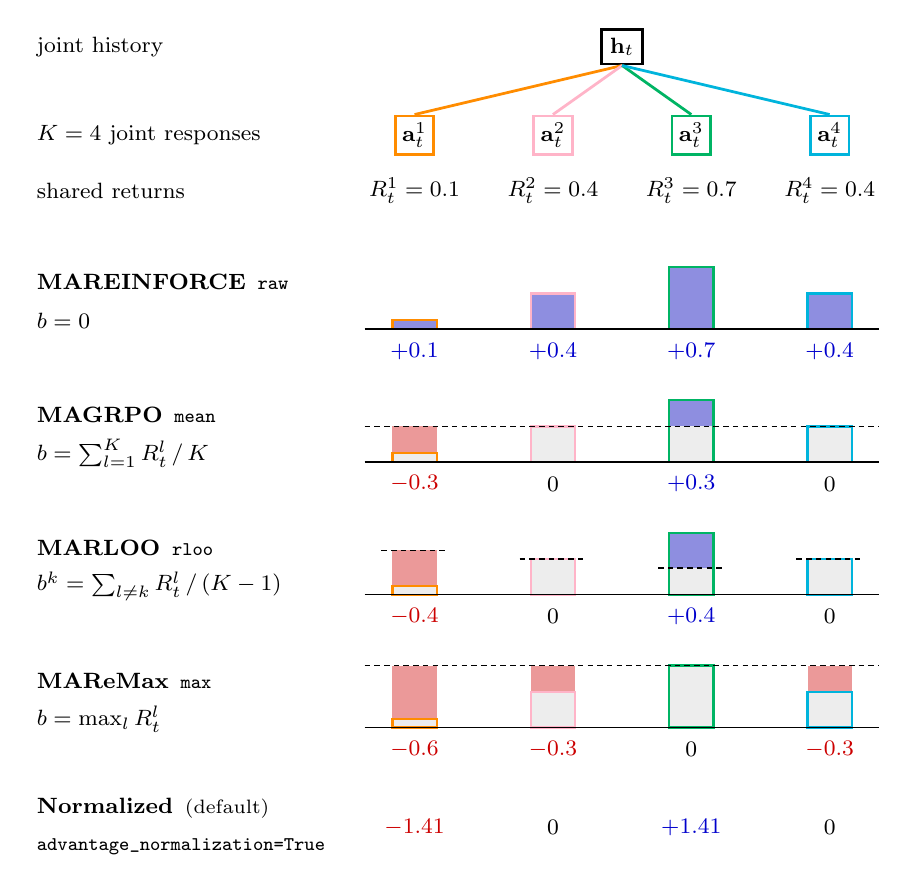
\begin{tikzpicture}[x=1pt, y=1pt, font=\footnotesize]
  % Stage 0: one joint history node.
  \node[draw, line width=1pt, inner sep=3pt] (h) at (215,0) {$\mathbf{h}_t$};
  \node[anchor=west] at (0,0) {joint history};

  % Stage 1: K = 4 sampled joint responses.
  \node[anchor=west] at (0,-32) {$K=4$ joint responses};
  \foreach \c [count=\i] in {s1,s2,s3,s4} {
    \pgfmathsetmacro{\x}{\colx[\i-1]}
    \node[draw=\c, line width=1pt, inner sep=2.5pt] (a\i) at (\x,-32) {$\mathbf{a}^{\i}_t$};
    \draw[\c, line width=1pt] (h.south) -- (a\i.north);
  }

  % Stage 2: the shared returns every agent receives.
  \node[anchor=west] at (0,-52) {shared returns};
  \foreach \r [count=\i] in {0.1,0.4,0.7,0.4} {
    \pgfmathsetmacro{\x}{\colx[\i-1]}
    \node at (\x,-52) {$R^{\i}_t=\r$};
  }

  % Stages 3-6: the same returns with each variant's baseline.
  \variantrow{-102}{MAREINFORCE}{raw}{$b=0$}{0,0,0,0}{}
  \variantrow{-150}{MAGRPO}{mean}{$b=\sum_{l=1}^{K}R^{l}_t\,/\,K$}{0.4,0.4,0.4,0.4}{0.4}
  \variantrow{-198}{MARLOO}{rloo}{$b^{k}=\sum_{l\neq k}R^{l}_t\,/\,(K-1)$}{0.5,0.4,0.3,0.4}{}
  \variantrow{-246}{MAReMax}{max}{$b=\max_{l}R^{l}_t$}{0.7,0.7,0.7,0.7}{0.7}

  % Stage 7: default advantage normalization.
  \node[anchor=west] at (0,-275) {\textbf{Normalized}\enspace{\scriptsize(default)}};
  \node[anchor=west] at (0,-289) {\scriptsize\ttfamily advantage\char95 normalization=True};
  \node[advneg] at (140,-282) {$-1.41$};
  \node at (190,-282) {$0$};
  \node[advpos] at (240,-282) {$+1.41$};
  \node at (290,-282) {$0$};
\end{tikzpicture}
\end{document}
